\documentclass[5p]{elsarticle} %review=doublespace preprint=single 5p=2 column
%%% Begin My package additions %%%%%%%%%%%%%%%%%%%
\usepackage[hyphens]{url}

  \journal{An awesome journal} % Sets Journal name

\sloppy

\usepackage{lineno} % add

\usepackage{graphicx}
%%%%%%%%%%%%%%%% end my additions to header

\usepackage[scaled]{helvet}

% Für die Schriftart Helvecia
\renewcommand*\familydefault{\sfdefault} 



\usepackage[T1]{fontenc}
\usepackage{lmodern}
\usepackage{amssymb,amsmath}
\usepackage{ifxetex,ifluatex}
\usepackage{fixltx2e} % provides \textsubscript
% use upquote if available, for straight quotes in verbatim environments
\IfFileExists{upquote.sty}{\usepackage{upquote}}{}
\ifnum 0\ifxetex 1\fi\ifluatex 1\fi=0 % if pdftex
  \usepackage[utf8]{inputenc}
\else % if luatex or xelatex
  \usepackage{fontspec}
  \ifxetex
    \usepackage{xltxtra,xunicode}
  \fi
  \defaultfontfeatures{Mapping=tex-text,Scale=MatchLowercase}
  \newcommand{\euro}{€}
\fi
% use microtype if available
\IfFileExists{microtype.sty}{\usepackage{microtype}}{}
\bibliographystyle{elsarticle-harv}
\ifxetex
  \usepackage[setpagesize=false, % page size defined by xetex
              unicode=false, % unicode breaks when used with xetex
              xetex]{hyperref}
\else
  \usepackage[unicode=true]{hyperref}
\fi
\hypersetup{breaklinks=true,
            bookmarks=true,
            pdfauthor={},
            pdftitle={Exploring an economical approach to the construction of a forest microclimate model},
            colorlinks=false,
            urlcolor=blue,
            linkcolor=magenta,
            pdfborder={0 0 0}}
\urlstyle{same}  % don't use monospace font for urls

\setcounter{secnumdepth}{5}
% Pandoc toggle for numbering sections (defaults to be off)


% tightlist command for lists without linebreak
\providecommand{\tightlist}{%
  \setlength{\itemsep}{0pt}\setlength{\parskip}{0pt}}


% Pandoc citation processing
\newlength{\cslhangindent}
\setlength{\cslhangindent}{1.5em}
\newlength{\csllabelwidth}
\setlength{\csllabelwidth}{3em}
\newlength{\cslentryspacingunit} % times entry-spacing
\setlength{\cslentryspacingunit}{\parskip}
% for Pandoc 2.8 to 2.10.1
\newenvironment{cslreferences}%
  {}%
  {\par}
% For Pandoc 2.11+
\newenvironment{CSLReferences}[2] % #1 hanging-ident, #2 entry spacing
 {% don't indent paragraphs
  \setlength{\parindent}{0pt}
  % turn on hanging indent if param 1 is 1
  \ifodd #1
  \let\oldpar\par
  \def\par{\hangindent=\cslhangindent\oldpar}
  \fi
  % set entry spacing
  \setlength{\parskip}{#2\cslentryspacingunit}
 }%
 {}
\usepackage{calc}
\newcommand{\CSLBlock}[1]{#1\hfill\break}
\newcommand{\CSLLeftMargin}[1]{\parbox[t]{\csllabelwidth}{#1}}
\newcommand{\CSLRightInline}[1]{\parbox[t]{\linewidth - \csllabelwidth}{#1}\break}
\newcommand{\CSLIndent}[1]{\hspace{\cslhangindent}#1}


\usepackage{diagbox}
\usepackage{makecell}

\begin{document}


\begin{frontmatter}

  \title{Exploring an economical approach to the construction of a forest microclimate model}
    \author[Philipps-University Marburg]{Thomas Beier}
   \ead{Beierth@students.uni-marburg.de} 
    \author[Philipps-University Marburg]{Florian Franz}
   \ead{Franzf@students.uni-marburg.de} 
    \author[Philipps-University Marburg]{Konstantin Seeger}
   \ead{Seegerk@students.uni-marburg.de} 
      \address[Philipps-University Marburg]{Philipps-University Marburg,
FB 19 Geography, Deutschhausstraße 10, 35032 Marburg, Germany}
    
  \begin{abstract}
Forests provide climate-regulating functions and are therefore important ecosystems in the context of climate change. In addition to forests acting as CO$_{2}$ sinks, their canopy can buffer temperature extremes, leading i.a. to lower temperatures in the forest than on exposed open spaces. This special microclimate provides refugia for many species. To identify such microrefugia, valid models of forest microclimates are needed. In recent years, much attention has been paid to microclimate modeling using predictors derived from Light Detection and Ranging (LiDAR) data and point-based measurements from data loggers as response. However, it is barely discussed how many point-based data loggers are needed for a valid prediction. In this study, we explored an economical approach to the construction of a forest microclimate model using LiDAR data and a varying number of loggers to determine a cost-effective model. Our results revealed a general decrease in prediction quality with fewer data loggers used for training. However, we saw that equal results could be achieved with fewer, more sensibly positioned loggers than with sheer logger quantity. We concluded that the positioning of the loggers is much more important than simply having a higher quantity to accurately model microclimates within forests.

  \end{abstract}
   \begin{keyword} Microclimate, Economical approach, \emph{TreeTalker}, Temperature, LiDAR, Random forest prediction \end{keyword}
 \end{frontmatter}

\newpage

\hypertarget{introduction}{%
\section{Introduction}\label{introduction}}

\graphicspath{ {./figures/} }

\begin{figure*}[t]
\begin{center}
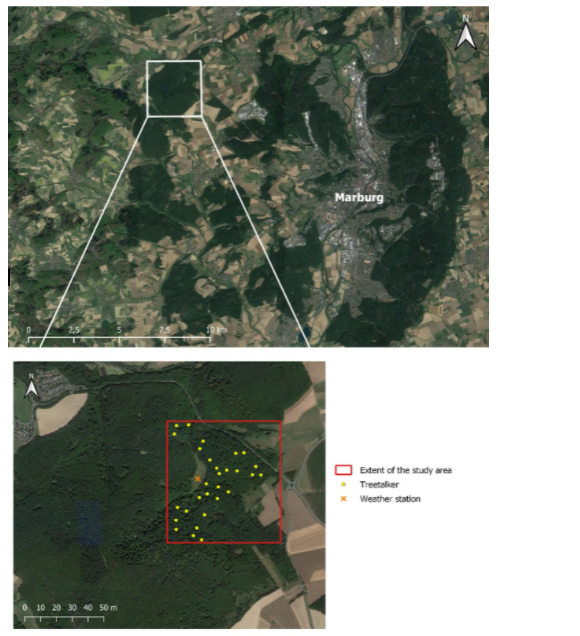
\includegraphics[scale=0.8]{study_area}
\caption{Location of the MOF (white square) and extent of the study area with locations of the \emph{TreeTalker} sensors and the weather station.}
\end{center}
\end{figure*}

The terms microclimate and micrometeorological scale range describe all climatic conditions of an area close to the earth’s surface, including atmospheric processes with a horizontal extension of up to 100 meters (Chen et al. 1999, DWD 2022, Foken 2006). Meteorological variables such as temperature, radiation, wind speed, and moisture are strongly influenced by the ground surface and vegetation cover, promoting forests to create a special microclimate (Chen et al. 1999, De Frenne et al. 2019, Zellweger et al. 2020). This microclimate within forest stands considerably differs from that in free, open landscapes (Bramer et al. 2018, Chen et al. 1999, De Frenne et al. 2019, De Frenne et al. 2021). Depending on their structure, canopy cover, macroclimate, and local water balance, forests have the potential to mitigate global warming impacts (Aussenac 2000, Davis et al. 2019a, De Frenne et al. 2019, Ehbrecht et al. 2019). These climatically buffered conditions provide microrefugia for many species as macroclimatic extremes increase in scale and frequency (Lenoir et al. 2017, Scheffers et al. 2014). Considering the broad impacts of anthropogenic climate change on biodiversity (Scheffers et al. 2016), it is crucial to identify such climatic microrefugia to possibly declare them as protected areas (Keppel et al. 2012, Keppel et al. 2015). For this purpose, microclimatic models can be helpful, as they allow a spatiotemporal prediction of climatic conditions on a small scale (Frey et al. 2016, Meineri \& Hylander 2017).\\
Several studies have been conducted on forest microclimate modeling (e.g. Frey et al. 2016, George et al. 2015, Greiser et al. 2018, Vanwalleghem \& Meentemeyer 2009). Machine learning approaches that use a certain number of predictors and one or more response variables are widely used in this context (Frey et al. 2016, George et al. 2015, Greiser et al. 2018). Meteorological parameters such as temperature or humidity measured by data loggers commonly serve as response variables (Frey et al. 2016). The predictors often include several forest structure related variables, as they have been shown to substantially influence the microclimate (Kovács et al. 2017). In recent years, progress in remote sensing technology, especially with Light Detection and Ranging (LiDAR) systems, has significantly enhanced microclimate modeling and mapping due to their ability to measure mentioned structural forest characteristics (Zellweger et al. 2019). LiDAR systems are active sensors which emit laser pulses in the near-infrared spectrum to measure the distance to a target, typically the earth’s surface (Wulder et al. 2008). Airborne laser scanning (ALS), referring to the generation of 3-dimensional point clouds with aircraft-mounted LiDAR instruments, is highly useful in forest research, as it enables an accurate derivation of horizontal and vertical information (Beland et al. 2019, Lim et al. 2003, Wulder et al. 2008, Zellweger et al. 2019). Such LiDAR derived metrics could be, for example, canopy height, Leaf Area Index (LAI), or biomass (Lim et al. 2003, Wulder et al. 2008). These metrics characterize forest stand structure and thus are well suited for predicting microclimate (Davis et al. 2019b, del Río et al. 2016, Zellweger et al. 2019).\\
Despite the widespread approach of using point-based measurements as response variables, it still remains an open question how many such points (or data loggers) are needed for a valid prediction of microclimate. However, producing a cost-effective model requires knowledge of the minimum viable number of response measurement points. Hence, we explored an economical approach to the construction of a forest microclimate model for the Marburg Open Forest (MOF) near the city of Marburg (Hesse, Germany). Our objective was to determine the minimum viable amount of point measurements for a valid prediction of the temperature under forest canopy, based on a random forest machine learning approach using LiDAR data for model training. We further investigated how the omission of loggers affected the prediction of other loggers. Our results may provide useful information on how to conduct future studies on microclimate modeling in a more cost-effective way.



\hypertarget{materials-and-methods}{%
\section{Materials and Methods}\label{materials-and-methods}}

\hypertarget{study-area}{%
\subsection{\texorpdfstring{Study area\\
}{Study area }}\label{study-area}}

The study was conducted in the university-owned “Calderner Forst”, also called “MOF”, 7 km northwest of Marburg (Fig. 1). It is roughly located at 50° 50’ 25.8’’ N and 8° 40’ 59.52’’ E with an elevation ranging between 233 m and 411 m above sea level. The long term average temperature of 30 years (1991 - 2020) in the region is 9.7 °C, the average long term annual precipitation 732 mm (HLNUG 2022, meteorological station Cölbe; 50° 85' N, 8° 77' E; 182 m above sea level). The MOF is a mixed forest stand mainly dominated by beech, oak, alder and spruce. Furthermore, a meadow (“Grubenwiese”) featuring a weather station is located amidst the tree stand. The whole area is used for various research activities by different universities. This study was focussed on an extent in the northeast of the MOF, covering an area of 55 ha (Fig. 1).


\hypertarget{data}{%
\subsection{\texorpdfstring{Data\\
}{Data }}\label{data}}

To derive the predictor variables, LiDAR data with an extent of the red square in Fig. 1 provided by the “Hessische Landesamt für Naturschutz, Umwelt und Geologie” was used (HLNUG 2018). The aerial survey at which it was recorded took place in spring 2018 under leafless conditions with a \emph{Riegl LMS-Q780} sensor. As response variable, temperature measurements from \emph{TreeTalker} sensors (TT+ 3.3 version, NATURE 4.0 SB SRL 2022) were used. In total, about 100 \emph{TreeTalkers} are installed in the MOF, 29 of which are located within the extent of our study area (Fig. 1). However, during the investigated period from June to August 2020, data was only available for 18 of them. Additionally to the \emph{TreeTalker} sensors, data from the weather station on the meadow was used. The station records 30 climate parameters and started operating in June 2017 (LCRS 2022). Its exact position is marked in Fig. 1.


\hypertarget{predictors}{%
\subsection{\texorpdfstring{Predictors\\
}{Predictors }}\label{Predictors}}

Generally, data management and processing was performed in the script language R in RStudio (R Core Team 2022). To process the raw LiDAR data, the \emph{lidR} package by Roussel et al. (2022) was used. Before the metrics could be calculated, the point cloud was normalized using inverse distance weighting as an algorithm for spatial interpolation (Roussel et al. 2021, Roussel et al. 2020).\\  
Afterwards, a total of 67 predictors were derived from the raw data on a 1 meter grid level (Tab. 1). 56 out of these are part of the standard metrics calculated in the \emph{lidR} package. The standard metrics are a collection of commonly used statistics like i.a. the mean height or mean intensity (Roussel et al. 2022). The Canopy Height Model (CHM) was calculated using a pit-free algorithm (Khosravipour et al. 2014), including 2, 5, 10, and 15 m as height thresholds for triangulations of first returns and a maximum edge of 1.5 (Roussel et al. 2021, Roussel et al. 2020). The LAI was calculated using the \emph{canopyLazR} package (Kamoske et al. 2019). Once again, we used inverse distance weighting to generate a Digital Terrain Model (DTM), taking the 6 closest neighbors with a power of 2 into account (Roussel et al. 2021, Roussel et al. 2020). Subsequently, the DTM was used to calculate slope, aspect, and Topographic Position Index (TPI) with the corresponding built-in functions of the \emph{raster} package by Hijmans et al. (2022). The first return metrics as well as point and pulse density were calculated with functions found in Roussel et al. (2021) and self-defined formulas, respectively.\\ 
Many of the 67 predictors have already been proven in other studies about microclimate modeling (e.g. Carrasco et al. 2019, Bennie et al. 2008, Hardiwck et al. 2014). A good overview can be found in Carrasco et al. (2019), who provided a matrix displaying correlations between LiDAR derived metrics and temperature. However, since all of the LiDAR predictors were static, only 18 unique values for each one were available as training data, leading to poor model performance. Hence, all the climate parameters from the weather station on the meadow were also added as predictors.


\hypertarget{model creation and validation}{%
\subsection{\texorpdfstring{Model creation and validation\\
}{Model creation and validation }}\label{model-creation-and-validation}}

All of the LiDAR predictors were stacked in a rasterStack using the \emph{raster} package. Afterwards, the pixel information from said stack corresponding with the \emph{TreeTalker} positions were extracted and combined with the hourly recorded climate variables from the \emph{TreeTalkers} and the weather station in a data frame. The next step was to remove NA-values and balance the data so an equal amount of measurements was used from each logger. This was done to avoid bias. The cleaning of the data frame continued by removing near-zero values and correlated predictors with a cutoff value of 0.9.\\ 
For validation purposes, the data frame was split into training and test data in a 80 to 20 ratio using the \emph{caret} package (Kuhn et al. 2022). Furthermore, the pixel-point of the weather station on the meadow was used as independent data to spatially validate the different models. Next, a function was created that randomly removed a specified amount of loggers, calculated a random forest ranger model from the remaining ones, predicted the temperature and saved the root-mean-square error (RMSE) for each \emph{TreeTalker} and the weather station. The results of each model run were cross-validated three times to create more accurate predictions. Hyperparameter tuning was applied with the combination of \emph{mtry} = 5 to 10, \emph{splitrule} = “extratrees” and \emph{min.node.size} = 5,10 or 15. The function was designed to remove the same amount of loggers five times, starting with 1 and ending with 17. Finally, the performance of the models created in the different function runs was compared based on the RMSE at the weather station and the \emph{TreeTalker} loggers.

\begin{table}[!h]
\renewcommand{\arraystretch}{2}
\begin{center}
\caption{LiDAR-derived metrics used as predictors.}
\scalebox{0.8}{
 \begin{tabular}{l  l  c  l} 
 \hline
 \\
 \textbf{Name} & \textbf{References} \\ [1ex]
 \hline
 CHM & Carrasco et al. 2019 \\ [1.5ex]
 
 First return metrics (mean/max/std) & Carrasco et al. 2019 \\ [1.5ex]

 Point density & Roussell et al. 2021 \\ [1.5ex]

 Pulse density & Roussell et al. 2021 \\ [1.5ex]
 
 LAI & \makecell[l]{Hardwick et al. 2014,\\ 
 Roth et al. 2020,\\ 
 Kamoske et al. 2019} \\ [1.5ex]
 
 DTM & \makecell[l]{George et al. 2015,\\ Latif 2012} \\ [1.5ex]
 
 Slope & Bennie et al. 2008 \\ [1.5ex]
 
 Aspect & Bennie et al. 2008 \\ [1.5ex]
 
 TPI & Ivajnšič et al. 2014 \\ [1.5ex]
 
 Standard metrics (n = 56) & Roussell et al. 2021 \\ [1.5ex]
 
 \hline
 \end{tabular}}
 \end{center}
\end{table}

\hypertarget{results}{%
\section{Results}\label{results}}

\begin{figure}[!ht]
\begin{center}
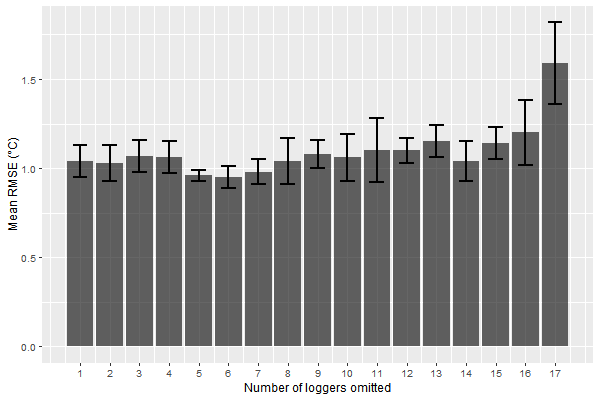
\includegraphics[scale=0.48]{rmse_wiese_mean_barplot}
\caption{Mean RMSE with error bars calculated for the position of the weather station on the meadow.}
\end{center}
\end{figure}

\begin{figure}[!h]
\begin{center}

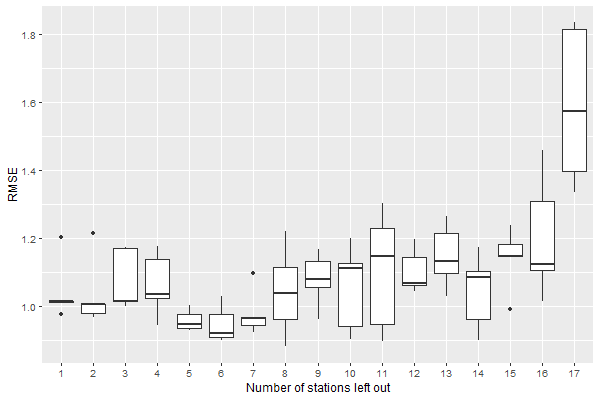
\includegraphics[scale = 0.48]{rmse_wiese_boxplot}
\caption{Boxplots of the RMSE calculated for the position of the weather station on the meadow.
}
\end{center}
\end{figure}

\begin{figure}[!h]
\begin{center}

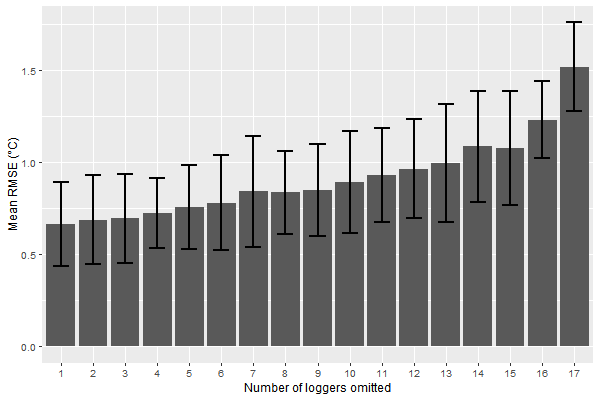
\includegraphics[scale = 0.48]{mean_rmse_gesamt_barplot}
\caption{Mean RMSE with error bars calculated for the position of the \emph{TreeTalker} loggers.}
\end{center}
\end{figure}

After cleaning the data frame, only 46 predictors remained. 11 of them were parameters from the weather station on the meadow, while the rest were LiDAR metrics. \\
Fig. 2 shows the mean RMSE including standard deviation of the predictions at the weather station in dependence on an increasing number of loggers omitted from the training data. Fig 3. displays the same data as boxplots. Both figures show a general trend of predictions improving with fewer loggers removed from the training dataset. However, the difference in RMSE between omitting few to omitting almost all of the loggers was not too great. In fact, when removing 5, 6 or 7 sensors, the mean and median RMSE dipped below 1.0 °C, lower than the RMSE of the prediction by the model with only 1 or 2 \emph{TreeTalkers} removed. The whiskers of the boxplots show that even with 14 or 15 loggers removed, an RMSE of less than 1.0 °C was achievable. Only with 17 sensors omitted, a clear increase in the RMSE was visible. \\
While analyzing all of the 85 function runs, it was noticed that in each of the 19 runs featuring the lowest meadow-RMSE, at least 4 loggers were omitted. The 20th best performing one was the first to remove less than 4 \emph{TreeTalkers}. Additionally, in three cases less than 4 loggers were removed in the worst twenty runs.\\
Fig. 4 displays an alternative validation approach averaging each \emph{TreeTalker} position’s RMSE in relation to the amount of loggers omitted. Fig. 5 shows the affiliated heatmap. As with the validation via the weather station, the RMSE increased with the number of loggers removed from the training data. The lowest RMSE values of around 0.4 °C occured when only 1 or 2 \emph{TreeTalkers} were omitted. Once again, some of the positions displayed low RMSEs of around 0.8 °C, even with 13, 14 or 15 loggers left out. Fig. 5 further demonstrates that even with only a single \emph{TreeTalker} sensor omitted, merely around half of the positions were predicted well, while the remaining ones featured slightly worse or way worse RMSE values. Especially \emph{TreeTalkers} 12 and 28’s temperatures were not well predicted. Both of them showed RMSE values of around 1.0 °C with only a single logger left out. Furthermore, removing less than 8 loggers did not lead to any further decrease in RMSE.\\ 
Fig. 6. exemplary shows the effect of the omission of loggers on the spatial prediction result for 12/06/2020 at 6 pm. With few training data removed, maximum temperatures of close to 22 °C were observed in certain parts of the predictions. Meanwhile modeled temperatures barely exceeded 21 °C, when a higher number of loggers was left out. When removing 17, i.e. all but 1 sensor, the same value was predicted for the whole study area.



\begin{figure*}[h]
\begin{center}
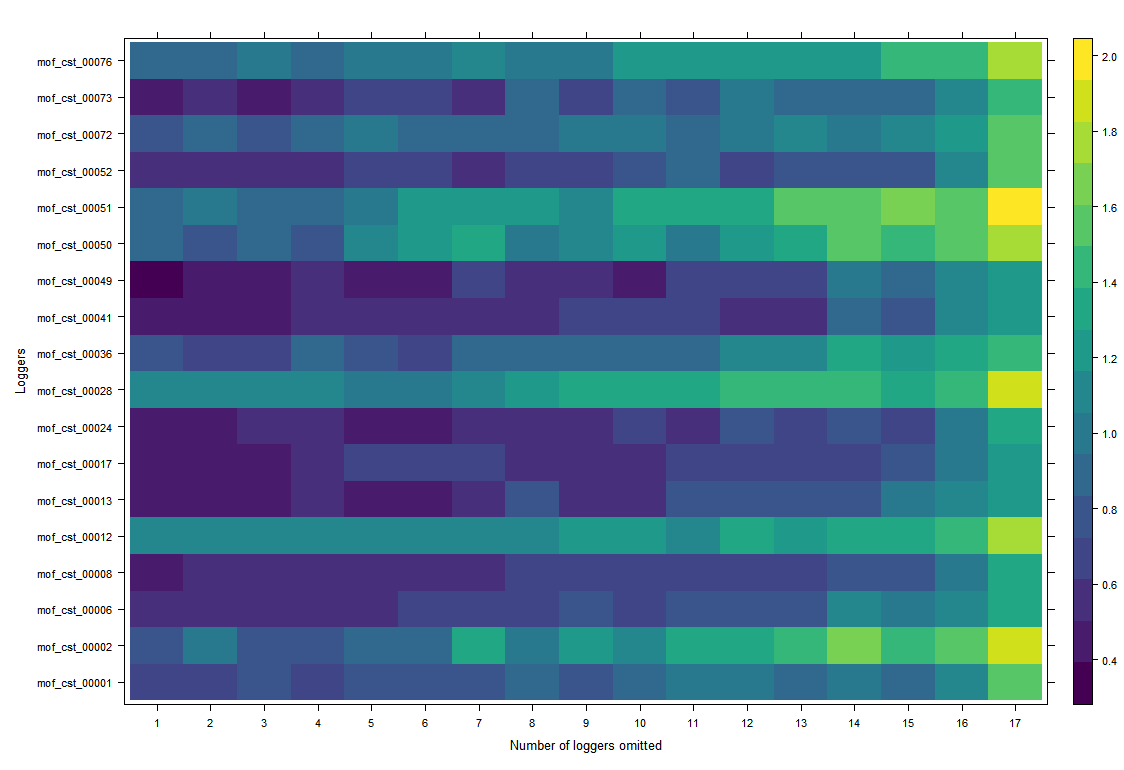
\includegraphics[scale=0.5]{heatmap_treetalker_rmse}
\caption{RMSE change of each \emph{TreeTalker} position with increasing number of removed loggers.}
\end{center}
\end{figure*}

\begin{figure*}[t]
\begin{center}
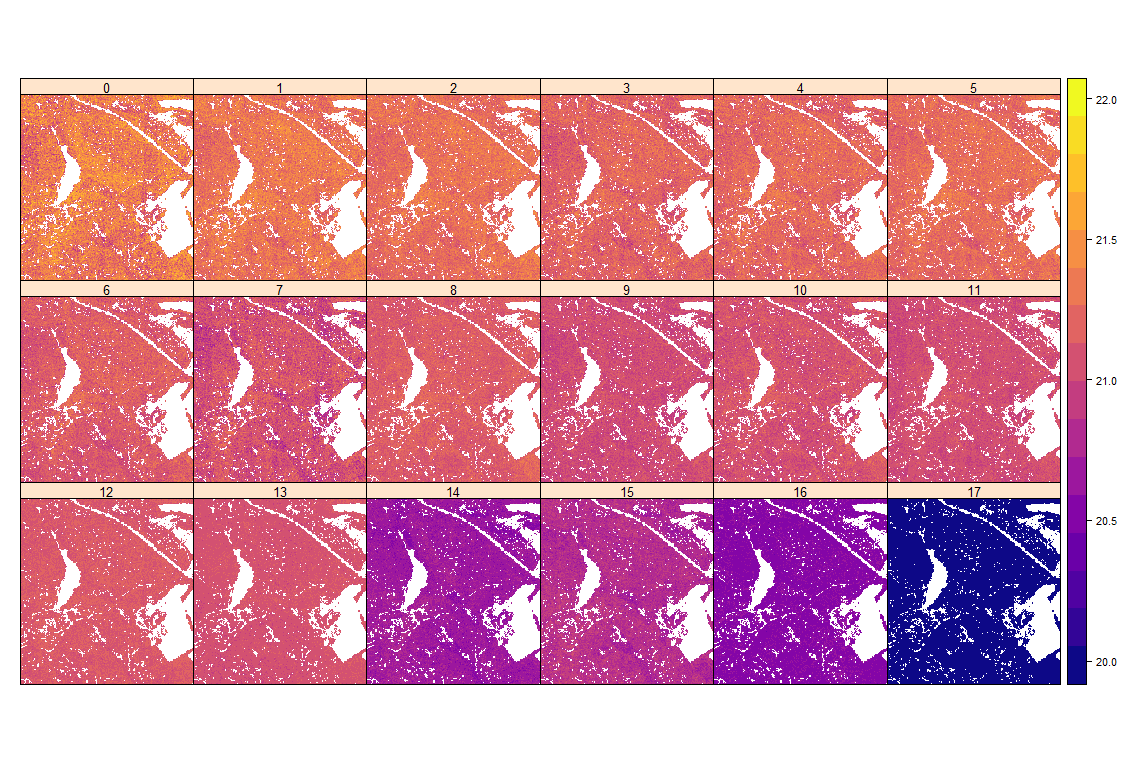
\includegraphics[scale=0.5]{full_prediction_study_area}
\caption{Temperature prediction (°C) of the study area for 12/06/2020 at 6 pm with an increasing number of loggers omitted.
}
\end{center}
\end{figure*}

\hypertarget{discussion}{%
\section{Discussion}\label{discussion}}

As expected, our results revealed a general trend of decreasing prediction quality with an increasing number of loggers left out, even though the meadow-RMSE values between few omitted \emph{Treetalkers} (1 or 2) and more omitted stations (13 or 14) differed by merely about 0.2 °C. Only when 17 loggers were left out, meaning soley 1 single logger was used for model training, a more significant decrease in the meadow-RMSE was noticeable. This was simply caused by the fact that no location specific predictors (topography, LiDAR), and only the temporal variations could be used for training the model. In contrast, Fig. 6 shows that despite the low variation of the meadow-RMSE, significant changes in the spatial distribution of the temperature prediction did in fact occur and a much finer distinction between temperature zones was possible with more loggers used for training. The dichotomy between the barely varying RMSE and the major changes in the prediction map makes sense, as our method of validation was only based on the single pixel of the weather station on the meadow out of the 550 000 pixels (= 0.0000018 \%) of the prediction result. Even if all 17 loggers were used for validation, it would still be lacking (= 0.00003 \%). This demonstrates that the RMSE derived from the meadow station alone was not a suitable measure to judge the spatial prediction quality. In short, while our models were able to predict the temperature quite well and accurately for certain positions at any time of the day, other positions were modeled worse, leading to a spatial inconsistency in prediction quality. 
When calculating the RMSEs for each individual location in dependence on an increasing number of loggers removed (Fig. 5), several positions’ temperature was predicted well even if up to 15 stations were left out. Other locations showed a much worse result. This was particularly evident for loggers 12 and 28. This means those two locations could not be predicted well by the training data from the other loggers because they most likely featured a property unique to them. Henceforth, these two loggers were crucial for a valid spatial temperature prediction in our study area. The best function runs always occurred when loggers 12 and 28 were included or only one of them was omitted. This also explains the low meadow-RMSE values even if 14 or 15 loggers were left out.\\  
Our results therefore suggest that it may be possible to achieve a prediction of equal or better quality with fewer loggers by selecting the “right” positions in the model training process. This is also well demonstrated in Fig. 2 and 3, where model predictions with 5, 6, 7 and 14 loggers left out partly show a lower and more consistent meadow-RMSE than model predictions that included training data from more loggers. Again, these results should be seen critically due to the subpar means of validation via the meadow-RMSE. After all, it could simply be the case that the runs that produced this rather good result used logger locations which were coincidentally well suited to predict the climate on the meadow, but not the rest of the forest. In fact, when taking a look at Fig. 4, where the mean RMSE of the individual locations is displayed, the seemingly better performance of those models is no longer apparent. Instead, the ones at which 8 and 15 locations were left out performed slightly better than their next lower counterparts. It needs to be added that there is a small bias because only 5 different combinations were run for each amount of omitted loggers. Theoretically, more function runs could have been performed. However, this would have been very time consuming, as  constructing models while removing only a low number of loggers took a lot of time. Putting these facts aside for now, the findings suggest that the selection of the loggers’ position seems to be much more important than their sheer number.\\ 
While we could not achieve our goal to identify a concrete minimum viable amount of response loggers, we found that it does not necessarily require many loggers, rather their sensible distribution in the modeled area to predict the different microclimates in a forest. To achieve the best result, the loggers should be positioned in a way that the training parameters are covered as heterogeneously as possible. In our example, a glaring observation was that despite a relatively high feature importance of the parameter “aspect”, not a single logger in our limited research area was positioned on a slope facing southwards.
Generally, not every scientific question involving microclimate modeling requires spatial accuracy as seen in the upper row of Fig. 6, e.g. when just comparing the temperatures within a forest to those outside (e.g. De Frenne et al. 2019). For these, even fewer loggers might be needed. However, such a fine distinction is especially relevant in ecological questions (e.g. Frey et al. 2016, Lembrechts et al. 2019), e.g. when mapping microrefugia for certain species.\\
To solidify and prove the results of this work, further research is recommended. Mainly it should be investigated which parameters cause certain locations to be well predicted. Respectively, it needs to be explored which variables are missing to accurately model locations that were represented poorly. Next, the research area could be expanded to cover the whole MOF, should the computing power be available. Furthermore, additional meteorological variables like humidity could be predicted. With further long-term research, a function to automatically select well-suited positions for the response loggers based on a raster stack of remotely sensed data (CHM, standard metrics, point and pulse density, LAI, Slope, Aspect, TPI…) could be developed. Such a function would be extremely useful and could provide a standardized and reproducible way of modeling large areas as economically, i.e. with as few loggers, as possible.



\hypertarget{conclusion}{%
\section{Conclusion}\label{conclusion}}

We created multiple microclimate models using a machine learning approach and airborne LiDAR data to predict temperature in a mixed forestry stand. Afterwards, the extent to which the omission of loggers influenced the prediction results was investigated.\\
We found that a decrease in positional training data did not manifest in a significant decrease in RMSE. Instead, spatial inconsistency in prediction quality increased, diminishing the explanatory power of our measure of validation. It was noted that spatial verifiability is a general problem inherent to raster-based microclimate modeling.\\ 
As expected, a general trend was found with the prediction quality improving when increasing the amount of \emph{TreeTalker} sensors. However, our results showed that it may be possible to reduce the number of loggers without sacrificing prediction quality. This can be achieved by planning their positions sensibly, covering the training parameters in the area as heterogeneously as possible. It is an effective way to reduce cost and expense when attempting to model larger areas. Furthermore, it is advised to adjust the number of loggers according to the scientific problem at hand. As a long term goal, it is proposed to develop a method to automatically locate optimal positions for the response loggers on the basis of remotely sensed data.

\hypertarget{references}{%
\section*{References}\label{references}}
\addcontentsline{toc}{section}{References}

\hypertarget{refs}{}
\begin{CSLReferences}{1}{0}


Beland, M., Parker, G., Sparrow, B., Harding, D., Chasmer, L., Phinn, S., Antonarakis, A. \& Strahler, A. (2019): On promoting the use of lidar systems in forest ecosystem research. \emph{For. Ecol. Manag.} 450, 117484.

Bennie, J., Huntley, B., Wilshire, A., O.Hill, M. \& Baxter R. (2008): Slope, aspect and climate: Spatially explicit and implicit models of topographic microclimate in chalk grassland. \emph{Ecol. Model.} 216 (1), 47-59.

Bramer, I., Anderson, B.J., Bennie, J., Bladon, A.J., De Frenne, P., Hemming, D., Hill, R.A., Kearney, M.R., Körner, C., Korstjens, A.H., Lenoir, J., Maclean, I.M.D., Marsh, C.D., Morecroft, M.D., Ohlemüller, R., Slater, H.D., Suggitt, A.J., Zellweger, F. \& Gillingham, P.K. (2018): Advances in monitoring and modelling climate at ecologically relevant scales. In: Bohan, D.A., Dumbrell, A.J., Woodward, G. \& Jackson, M. (Eds.): \emph{Adv. Ecol. Res.} 58. Next generation biomonitoring: part 1., 101-161.

Carrasco, L., Giam, X., Papeş, M. \& Sheldon, K.S. (2019): Metrics of Lidar-Derived 3D Vegetation Structure Reveal Contrasting Effects of Horizontal and Vertical Forest Heterogeneity on Bird Species Richness. \emph{Remote Sens.} 11 (7), 743.

Chen, J., Saunders, S.C., Crow, T.R., Naiman, R.J., Brosofske, K.D., Mroz, G.D., Brookshire, B.L. \& Franklin, J.F. (1999): Microclimate in Forest Ecosystem and Landscape Ecology. Variations in local climate can be used to monitor and compare the effects of different management regimes. \emph{BioScience} 49 (4), 288-297.

Davis, K.T., Dobrowski, S.Z., Holden, Z.A., Higuera, P.E. \& Abatzoglou, J.T. (2019a): Microclimatic buffering in forests of the future: the role of local water balance. \emph{Ecography} 42 (1), 1-11.

Davis, F.W., Synes, N.W., Fricker, G.A., McCullough, I.M., Serra-Diaz, J.M., Franklin, J. \& Flint, A.L. (2019b): LiDAR-derived topography and forest structure predict fine-scale variation in daily surface temperatures in oak savanna and conifer forest landscapes. \emph{Agric. For. Meteorol.} 269-270, 192-202.

De Frenne, P., Zellweger, F., Rodríguez-Sánchez, F., Scheffers, B.R., Hylander, K., Luoto, M., Vellend, M., Verheyen, K. \& Lenoir, J. (2019): Global buffering of temperatures under forest canopies. \emph{Nat. Ecol. Evol.} 3, 744-749.

De Frenne, P., Lenoir, J., Luoto, M., Scheffers, B.R., Zellweger, F., Aalto, J., Ashcroft, M.B., Christiansen, D.M., Decocq, G., Pauw, K.D., Govaert, S., Greiser, C., Gril, E., Hampe, A., Jucker, T., Klinges, D.H., Koelemeijer, I.A., Lembrechts, J.J., Marrec, R., Meeussen, C., Ogée, J., Tyystjärvi, V., Vangansbeke, P. \& Hylander, K. (2021): Forest microclimates and climate change: Importance, drivers and future research agenda. \emph{Glob. Change Biol.} 27 (11), 2279-2297.

Deutscher Wetterdienst (DWD) (2022): Mikroklima. \url{https://www.dwd.de/DE/service/lexikon/Functions/glossar.html?lv2=101640&lv3=101778} (Accessed on 28/03/2022).

Foken, T. (2006): Angewandte Meteorologie. Mikrometeorologische Methoden. 2. Auflage. Springer-Verlag. Berlin, Heidelberg.

Frey, S.J.K., Hadley, A.S., Johnson, S.L., Schulze, M., Jones, J.A. \& Betts, M.G. (2016): Spatial models reveal the microclimatic buffering capacity of old-growth forests. \emph{Sci. Adv.} 2 (4), e1501392.

George, A.D., Thompson, F.R. \& Faaborg, J. (2015): Using LiDAR and remote microclimate loggers to downscale near-surface air temperatures for site-level studies. \emph{Remote Sens.} Lett. 6 (12), 924-932.

Greiser, C., Meineri, E., Luoto, M., Ehrlén, J. \& Hylander, K. (2018): Monthly microclimate models in a managed boreal forest landscape. \emph{Agric. For. Meteorol.} 250-251, 147-158.

Hardwick, S.R., Toumi, R., Pfeifer, M., Turner, E.C., Nilius, R. \& Ewers R.M. (2014): The relationship between leaf area index and microclimate in tropical forest and oil palm plantation: Forest disturbance drives changes in microclimate. \emph{Agric. For. Meteorol.} 201, 187-195.

Hijmans, R.J., van Etten, J., Sumner, M., Cheng, J., Baston, D., Bevan, A., Bivand, R., Busetto, L., Canty, M., Fasoli, B., Forrest, D., Ghosh, A., Golicher, D., Gray, J., Greenberg, J.A., Hiemstra, P., Hingee, K., Ilich, A., Institute for Mathematics Applied Geosciences, Karney, C., Mattiuzzi, M., Mosher, S., Naimi, B., Nowosad, J., Pebesma, E., Lamigueiro, O.P., Racine, E.B., Rowlingson, B., Shortridge, A., Venables, Bill. \& Wueest, R. (2022): raster: Geographic Data Analysis and Modelling. R package version 3.5-11. \url{https://cran.r-project.org/web/packages/raster/index.html} (Accessed on 31/03/2022).

HLNUG (2018): Airbone Laserscanning. \url{https://hvbg.hessen.de/} (Accessed on 08/04/2022).

HLNUG (2022): Messwerte, Klimastation Cölbe. \url{https://www.hlnug.de/messwerte/witterungs-undklimadaten/wetterextreme} (Accessed on 09/04/2022).

Ivajnšič, D., Kaligarič M. \& Žiberna I. (2014): Geographically weighted regression of the urban heat island of a small city. \emph{Appl. Geogr.} 53, 341-353. 

Kamoske, A.G., Dahlin, K.M., Shawn, M.D \& Serbin, C.S. (2019): Leaf area density from airborne LiDAR: Comparing sensors and resolutions in a temperate broadleaf forest ecosystem. \emph{For. Ecol. Manag.} 433, 364-375.

Keppel, G., Van Niel, K.P., Wardell-Johnson, G.W., Yates, C.J., Byrne, M., Mucina, L., Schut, A.G.T., Hopper, S.D. \& Franklin, S.E. (2012): Refugia: identifying and understanding safe havens for biodiversity under climate change. \emph{Global Ecol. Biogeogr.} 21 (4), 393-404.

Keppel, G., Mokany, K., Wardell-Johnson, G.W., Phillips, B.L., Welbergen, J.A. \& Reside, A.E. (2015): The capacity of refugia for conservation planning under climate change. \emph{Front. Ecol. Environ.} 13 (2), 106-112.

Khosravipour, A., Skidmore, A.K., Isenburg, M., Wang, T. \& Hussin, Y.A. (2014): Generating Pit-free Canopy Height Models from Airborne Lidar. \emph{Photogramm. Eng. Remote Sens.} 80 (9), 863–872.

Kovács, B., Tinya, F. \& Ódor, P. (2017): Stand structural drivers of microclimate in mature temperate mixed forests. \emph{Agric. For. Meteorol.} 234-235, 11-21.

Kuhn, M., Wing, J., Weston, S., Williams, A., Keefer, C., Engelhardt, A., Cooper, T., Mayer, Z., Kenkel, B., R Core Team, Benesty, M., Lescarbeau, R., Ziem, A., Scrucca, L., Tang, Y., Candan, C. \& Hunt T. (2022):  caret: Classification and Regression Training. \url{https://cran.r-project.org/web/packages/caret/index.html} (Accessed on 31/03/2022).
 
Latif, Z.A. (2012): Forest Microclimate Modelling Using Remotely Sensed Data. \emph{ISrJ.} 2 (1), 19-25.

LCRS (2022): Caldern Klimastation Wiese. \url{http://lcrs.geographie.uni-marburg.de/lcrs/data_pre.do?citid=302} (Accessed on 29/03/2022).

Lembrechts, J.J., Nijs, I. \& Lenoir, J. (2019): Incorporating microclimate into species distribution models. \emph{Ecography} 42 (7), 1267-1279.

Lenoir, J., Hattab, T. \& Pierre, G. (2017): Climatic microrefugia under anthropogenic climate change: implications for species redistribution. \emph{Ecography} 40 (2), 253-266.

Lim, K., Treitz, P., Wulder, M., St-Onge, B. \& Flood, M. (2003): LiDAR remote sensing of forest structure. \emph{Prog. Phys. Geogr.} 27 (1), 88-106.

Meineri, E. \& Hylander, K. (2017): Fine-grain, large-domain climate models based on climate station and comprehensive topographic information improve microrefugia detection. \emph{Ecography} 40 (8), 1003-1013.

NATURE 4.0 SB SRL (2022): NATURE 4.0. Wireless systems for environment, agriculture and wildlife. \url{https://www.nature4shop.com/} (Accessed on 04/04/2022).

R Core Team (2022): The R Project for Statistical Computing. https://www.r-project.org/ (Accessed on 30/03/2022). 

Roth, D.B., Goodenough, A.A.,Brown, S.D., van AArdt, J.A., Saunders, M.G. \& Krause K. (2020): Simulations of Leaf BSDF Effects on Lidar Waveforms. \emph{Remote Sens.} 12 (18), 2909.

Roussel, J.-R., Auty, D., Coops, N.C., Tompalski, P., Goodbody, T.R.H., Sánchez Meador, A., Bourdon, J.-F., De Boissieu, F. \& Achim, A. (2020): lidR: An R package for analysis of Airborne Laser Scanning (ALS) data. \emph{Remote Sens. Environ.} 251, 112061.

Roussel, J.-R., Goodbody, T.R.H. \& Tompalski, P. (2021): The lidR package. \url{https://r-lidar.github.io/lidRbook/index.html} (Accessed on 29/03/2022).

Roussel, J.-R., Auty, D., De Boissieu, F., Sánchez Meador, A., Bourdon, J.-F., Demetrios, G., Steinmeier, L. \& Adaszewski, S. (2022): Package ‘lidR’. \url{https://cran.r-project.org/web/packages/lidR/index.html} (Accessed on 29/03/2022).

Scheffers, B.R., Edwards, D.P., Diesmos, A., Williams, S.E. \& Evans, T.A. (2014): Microhabitats reduce animal’s exposure to climate extremes. \emph{Glob. Change Biol.} 20 (2), 495-503.

Scheffers, B.R., De Meester, L., Bridge, T.C.L., Hoffmann, A.A., Pandolfi, J.M., Corlett, R.T., Butchart, S.H.M., Pearce-Kelly, P., Kovacs, K.M., Dudgeon, D., Pacifici, M., Rondinini, C., Foden, W.B., Martin, T.G., Mora, C., Bickford, D. \& Watson, J.E.M. (2016): The broad footprint of climate change from genes to biomes to people. \emph{Science} 354 (6313), aaf7671.

Vanwalleghem, T. \& Meentemeyer, R.K. (2009): Predicting Forest Microclimate in Heterogeneous Landscapes. \emph{Ecosystems} 12 (7), 1158-1172.

Wulder, M.A., Bater, C.W., Coops, N.C., Hilker, T. \& White, J.C. (2008): The role of LiDAR in sustainable forest management. \emph{For. Chron}. 84 (6), 807-826.

Zellweger, F., De Frenne, P., Lenoir, J., Rocchini, D. \& Coomes, D. (2019): Advances in Microclimate Ecology Arising from Remote Sensing. \emph{Trends Ecol. Evol.} 34 (4), 327-341.

Zellweger, F., De Frenne, P., Lenoir, J., Vangansbeke, P., Verheyen, K., Bernhardt-Römermann, M., Baeten, L., Hédl, R., Berki, I., Brunet, J., Van Calster, H., Chudomelová, M., Decocq, G., Dirnböck, T., Durak, T., Heinken, T., Jaroszewicz, B., Kopecký, M., Máliš, F., Macek, M., Malicki, M., Naaf, T., Nagel, T.A., Ortmann-Ajkai, A., Petřík, P., Pielech, R., Reczyńska, K., Schmidt, W., Standovár, T., Świerkosz, K., Teleki, B., Vild, O., Wulf, M. \& Coomes, D. (2020): Forest microclimate dynamics drive plant responses to warming. \emph{Science} 368, 772-775.


\end{CSLReferences}

\end{document}
